\documentclass[10pt, a4paper]{article}
% ===== Essential Packages =====
\usepackage[utf8]{inputenc}       % UTF-8 encoding
\usepackage[T1]{fontenc}          % Better font encoding
\usepackage{lmodern}              % Modern Latin Modern font
\usepackage{ctex}                 % Chinese support (must be loaded after fontenc)
\usepackage{subcaption}
% ===== Math & Symbols =====
\usepackage{amsmath}              % Advanced math
\usepackage{amssymb}              % Additional math symbols
\usepackage{mathrsfs}             % Ralph Smith's Formal Script
\usepackage{braket}               % Dirac bra-ket notation

% ===== Graphics & Tables =====
\usepackage{graphicx}             % Image support
\usepackage{float}                % Better float control
\usepackage{wrapfig}              % Wrapped figures
\usepackage{tikz}                 % Vector graphics
\usepackage[table]{xcolor}        % Colored tables
\usepackage{array}                % Enhanced tables
\usepackage{multirow}             % Multirow tables
\usepackage{tabularx}             % Adjustable-width tables
\usepackage{booktabs}             % Professional table lines
\usepackage{siunitx}              % SI units in tables
\usepackage{caption}              % Better captions
\usepackage{adjustbox}            % Box resizing

% ===== Code Listings =====
\usepackage{listings}             % Code blocks
\usepackage{tcolorbox}            % Colored boxes
\tcbuselibrary{listings, breakable} % Listings in tcolorbox

% ===== Misc =====
\usepackage{lipsum}               % Dummy text
\usepackage{footmisc}             % Better footnotes
\usepackage[margin=1in]{geometry} % Page margins
\usepackage{diagbox}
\usepackage{ctex}
\author{张世航}
\title{热电子发射}
\begin{document}
	\maketitle
	\section{逸出功的测量}
	\begin{tabular}{|c|c|c|c|c|c|c|c|}
		\hline
		\diagbox[width=3cm]{$I_f(A)$}{$I_a(\mu A)$}{$U_a(V)$} & 25 & 36 & 49 & 64 & 81 & 121 & 144 \\
		\hline
		0.58(1960K) & 14 & 14 & 14 & 14 & 15 & 15 & 15 \\
		\hline
		0.62(2030K) & 39 & 40 & 41 & 41 & 42 & 44 & 44 \\
		\hline
		0.64(2100K) & 64 & 64 & 65 & 66 & 67 & 69 & 70 \\
		\hline
		0.70(2170K) & 238 & 241 & 243 & 244 & 251 & 259 & 263 \\
		\hline
		0.74(2240K) & 514 & 521 & 535 & 544 & 550 & 584 & 592 \\
		\hline
		0.78(2310K) & 1069 & 1090 & 1105 & 1123 & 1132 & 1161 & 1178 \\
		\hline
	\end{tabular}\\
	由于\[lgI_a = lgI + \frac{0.439}{2.3T}\frac{\sqrt{U_a}}{\sqrt{r_1ln\frac{r_2}{r_1}}}\]
	\begin{figure}[H]
		\centering
		
\includegraphics[width=0.7\linewidth]{1}
		\label{fig:1}
	\end{figure}
	\begin{figure}[H]
		\centering
		
\includegraphics[width=0.7\linewidth]{2}
		\label{fig:2}
	\end{figure}
	可以计算得到逸出功为\[e\varphi = \frac{26186.1532}{5030}=5.20599eV\]
	查阅资料,标准值为$4.55 eV$
	相对误差为\[\frac{|5.20599eV-4.59 eV|}{4.59 eV}\times100\%=13.4\%\]
	\section{费米狄拉克分布}
	\scalebox{0.642}{
		\begin{tabular}{|c|c|c|c|c|c|c|c|c|c|c|c|c|c|c|c|c|c|c|c|c|c|}
			\hline
			$I_s(A)$ & 0.003 & 0.025 & 0.036 & 0.044 & 0.051 & 0.057 & 0.062 & 0.067 & 0.072 & 0.076 & 0.081 & 0.085 & 0.088 & 0.092 & 0.095 & 0.099 & 0.102 & 0.105 & 0.108 & 0.111 & 0.114 \\
			\hline
			$I_a(\mu A)$ & 42 & 40 & 38 & 36 & 34 & 32 & 29 & 25 & 22 & 19 & 14 & 11 & 8 & 5 & 4 & 2 & 2 & 1 & 1 & 1 & 0 \\
			\hline
		\end{tabular}
	}
	我们有\[\frac{I_a}{I_{a_0}} = \frac{1}{e^{\frac{K'I_s^2-\epsilon_F}{kT}}+1}\]
	我们的实验中没有准确的测得$I_{a_0}$的值,我下面的计算将会表明,$I_{a_0}$微小的测量误差将会导致费米能计算的较大的误差.\\
	我们可以将上式化简为\[I_s^2 = \frac{kT}{K'}ln(\frac{I_{a_0}}{I_a}-1)+\frac{\epsilon_F}{K'}\]
	对上面式子用最小二乘法拟合.\\
	我们可以列出一个表格,不同的$I_{a_0}$对应的不同的$\epsilon_F$.\\
		\scalebox{0.85}{
		\begin{tabular}{|c|c|c|c|c|c|c|c|c|c|c|c|c|}
			\hline
			$I_{a_0}(\mu A)$& 42.000000001 & 42.00000001 & 42.0000001 & 42.000001 & 42.00001 & 42.0001 & 42.001 & 42.01 & 42.1 & 42.2 & 42.3 & 42.4 \\
			\hline
			$\epsilon_F(eV)$& 2.88 & 2.58 & 2.29 & 2.02 & 1.76 & 1.54 & 1.34 & 1.16 & 1.02 & 0.98 & 0.96 & 0.95 \\
			\hline
		\end{tabular}
	}
	由于我们实验仪器的精度受到限制,我们无法进行准确的测量.所以无法准确计算费米能$\epsilon_F$\\
	面对这种情况,我们假设$r^2$最大的值接近真实的情况,我们可以采用梯度下降的方法找到一个最大的$r^2$来使我的实验数据拟合的最好.我们利用梯度下降的方法,计算出当$I_{a_0} = 42.2612\mu A$时,我们得到最大的$r^2 = 0.846198$.我们故且相信这是最接近真实情况的值.此时的$\epsilon_F = 0.9699215207244691eV$,$K' = 179.10002524405797eV/A^2$\\
	\begin{figure}[H]
		\centering
		\setlength{\tabcolsep}{2pt} % 减小列间距
		\begin{tabular}{cccc}
			
\includegraphics[width=0.23\textwidth]{1.1} &
			
\includegraphics[width=0.23\textwidth]{1.2} &
			
\includegraphics[width=0.23\textwidth]{1.3} &
			
\includegraphics[width=0.23\textwidth]{1.4} \\

			
			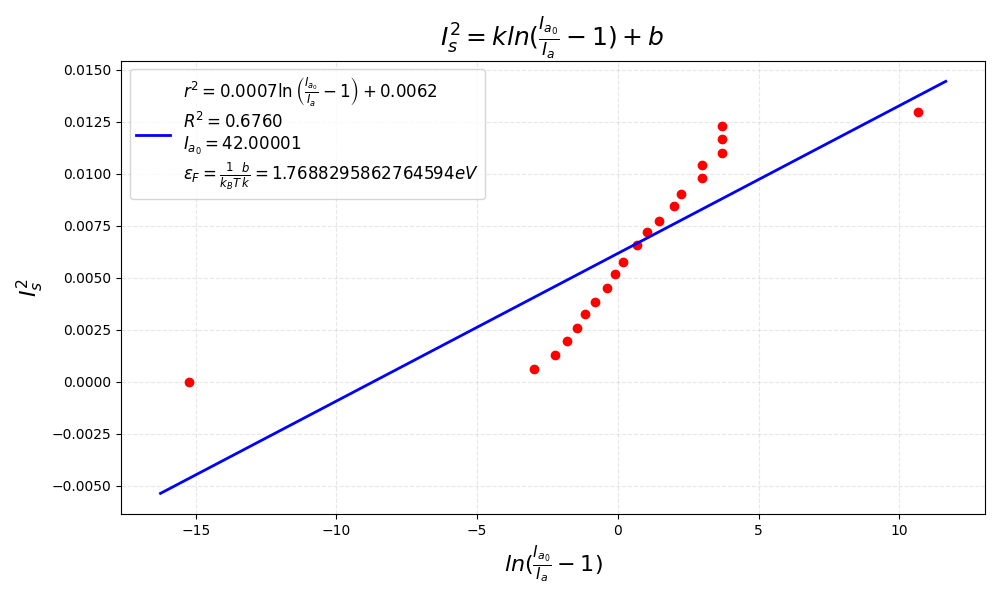
\includegraphics[width=0.23\textwidth]{1.5} &
			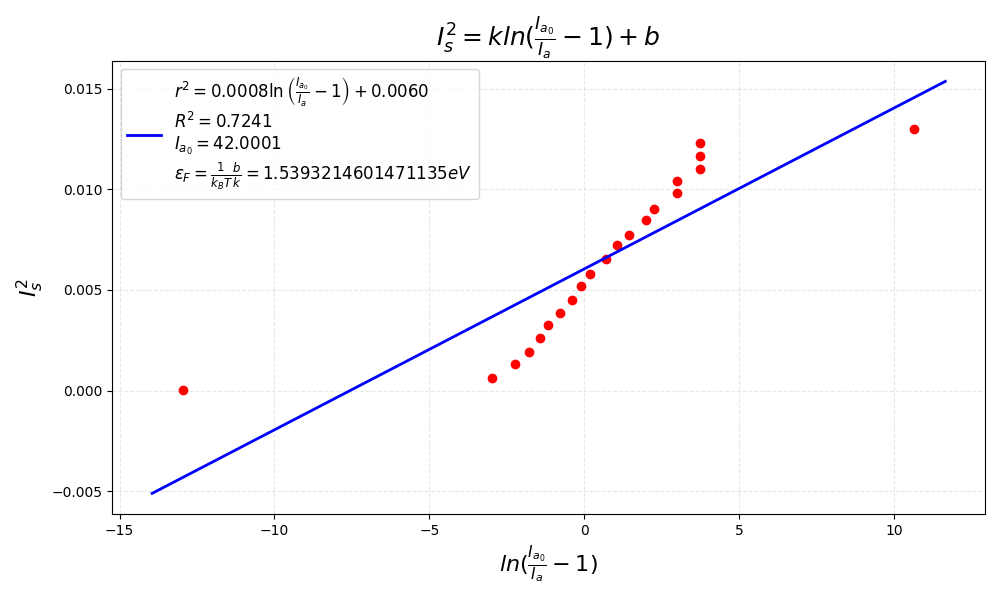
\includegraphics[width=0.23\textwidth]{1.6} &
			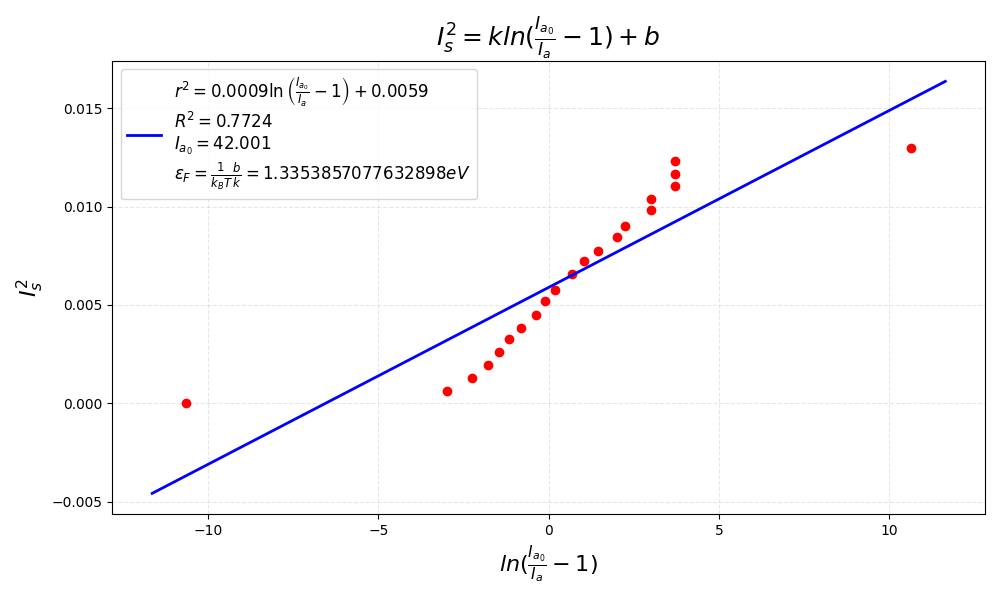
\includegraphics[width=0.23\textwidth]{1.7} &
			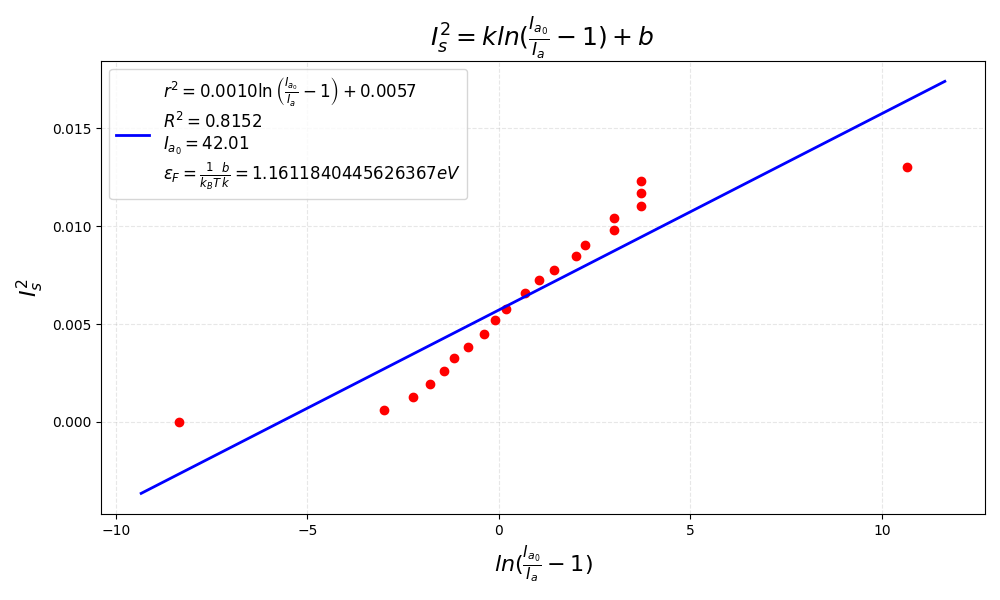
\includegraphics[width=0.23\textwidth]{1.8} \\

			
			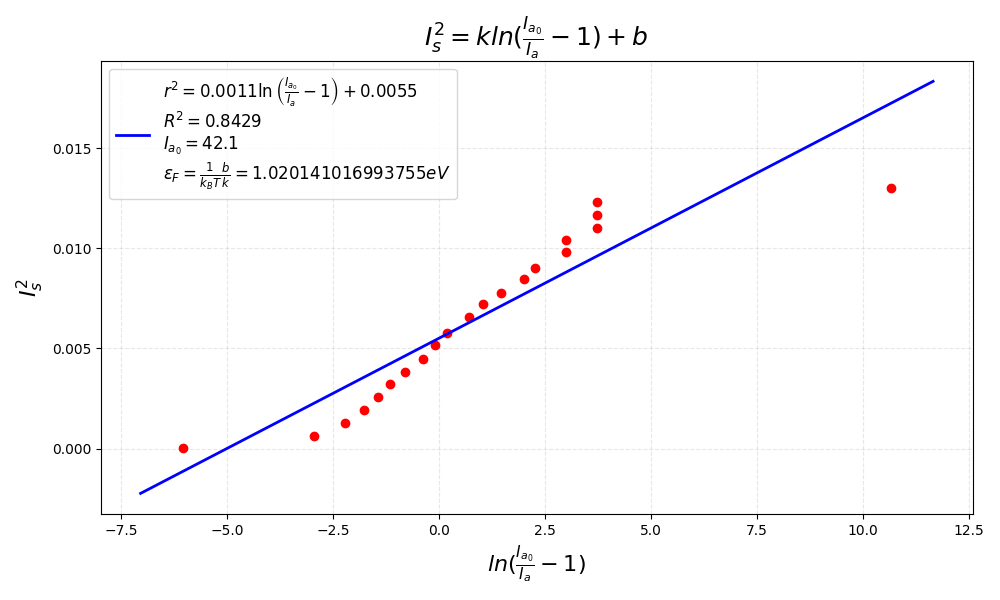
\includegraphics[width=0.23\textwidth]{1.9} &
			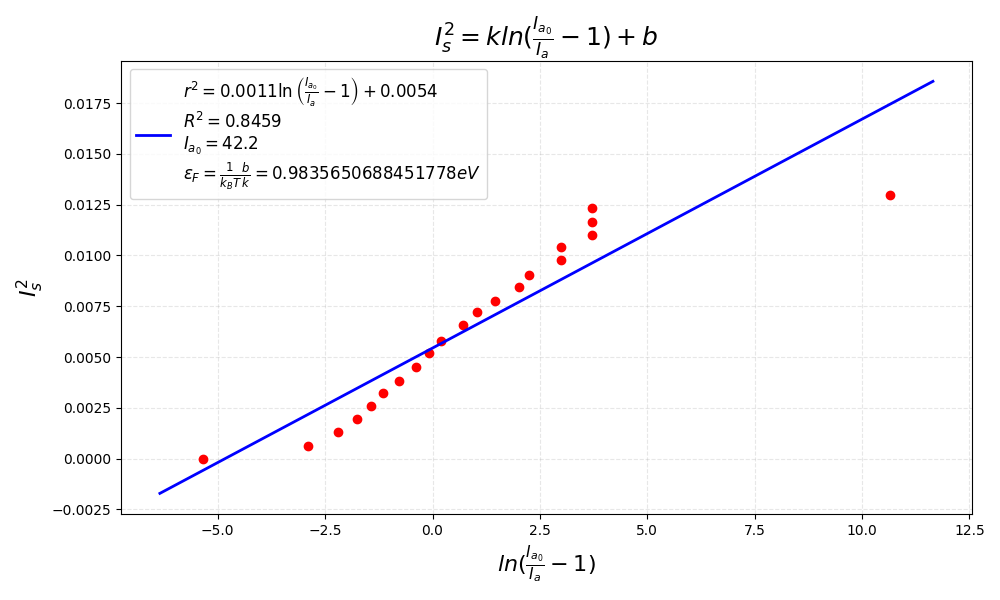
\includegraphics[width=0.23\textwidth]{2.0} &
			
\includegraphics[width=0.23\textwidth]{2.1} &
			
\includegraphics[width=0.23\textwidth]{2.2}  \\

		\end{tabular}
		\caption{不同$I_{a_0}$对应的不同的$\epsilon_F$}
	\end{figure}
	\begin{figure}[H]
		\centering
		
\includegraphics[width=0.65\linewidth]{3}
		\label{fig:3}
	\end{figure}
	\begin{figure}[H]
		\centering
		
\includegraphics[width=0.7\linewidth]{4}
		\label{fig:4}
	\end{figure}
	\[B = 2.95\times10^{-2}I_s T/A\]
	\[\frac{e}{m} = 1.096168193414791\times10^{11}C/kg\]
	\section{Richardson effect}
	金属表面单位面积,单位时间的电子的逸出数为
	\[R = \int_{p_z=(2mW)^\frac{1}{2}}^{\infty}\int_{p_x=-\infty}^{\infty}\int_{p_x=-\infty}^{\infty}\{\frac{2dp_xdp_ydp_z}{h^3}\frac{1}{e^{\epsilon-\mu}+1}\}u_z\]
	我们在柱坐标系中进行积分
	\begin{align*}
		R &= \frac{2}{h^3}\int_{p_z=(2mW)^\frac{1}{2}}^{\infty}\frac{p_z}{m}dp_z\int_{p'=0}^{\infty}\frac{2\pi p'dp'}{exp\{[\frac{p'^2}{2m}+\frac{p_z^2}{2m}-\mu]/kT\}+1}\\
		&=\frac{4\pi kT}{h^3}\int_{p_z=(2mW)^\frac{1}{2}}^{\infty}p_zdp_zln[1+exp\{\frac{\mu-\frac{p_z^2}{2m}}{kT}\}]\\
		&=\frac{4\pi mkT}{h^3}\int_{\epsilon_z=W}^{\infty}d\epsilon_zln[1+e^{(\mu-\epsilon_z)/kT}]\\
		&=-\frac{4\pi mk^2T^2}{h^3}\mathrm{PolyLog}\left[2, -e^{\frac{\mu - W}{k T}}\right]
	\end{align*}
	\begin{figure}[H]
		\centering
		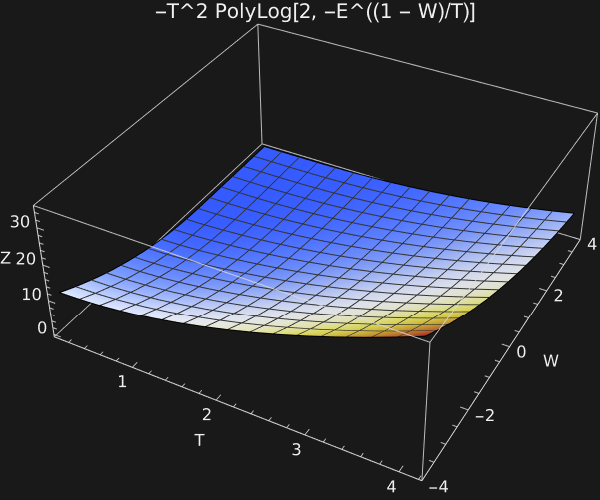
\includegraphics[width=0.7\linewidth]{3.1}

	\end{figure}
	
	精确积分是一个多对数函数积分的结果,为了得到Richardson公式,我们做进一步的化简.\\
	\[ln(1+x)\simeq x\]
	则\[R = \frac{4\pi mkT}{h^3}\int_{\epsilon_z=W}^{\infty}d\epsilon_ze^{\frac{\mu-\epsilon_z}{kT}}=\frac{4\pi mk^2T^2}{h^3}e^{\frac{(\mu-W)}{kT}}\]
	\[J = eR = \frac{4\pi mek^2T^2}{h^3}e^{\frac{(\mu-W)}{kT}}=\frac{4\pi mek^2T^2}{h^3}e^{-\frac{\varphi}{kT}}(\varphi=W-\epsilon_F)\]
	
	
\end{document} 